% Generated by documents/paper/figures/make_rq_appendix.py from the rq05_design_decisions README; do not edit.
\clearpage
\section{Design decisions}
\label{app:rq05_design_decisions}

\begin{rqfinding}
1. Per-language BPB of the trained languages reads the temperature decision from every proxy (0.95--0.99, mean over K15--K50) and the language-list decision at 0.77--1.00 (K8--K30), while on the gated benchmarks only one proxy reads a decision at 0.75 (the K1 DCLMP swap at 350M, 0.79): 0.41--0.62 for every intervention but the two K1 English-data swaps (DCLMP 0.50--0.79, FWEB 0.60--0.74). (Figure~\ref{fig:app_rq05_design_decisions}.)

2. On per-language BPB the temperature decision is read at 0.87--1.00 by every proxy at every K, and the language-list decision at 0.83--1.00 except 1B at K30 (0.31).

3. The depth decision on per-language BPB is 0.00 for 600M at all four K and 0.00--0.97 for 350M, while 90M, 175M and 1B read it at 0.78--1.00.
\end{rqfinding}

\paragraph{Question.} At a given number of languages K, when does a small model rank a design choice (depth, data scheme, temperature) the way the 1.7B reference does, and how does the answer move with K?

\paragraph{Setup.} Four single-axis interventions against the deep, scheme-A, $T = 1$ baseline: depth (deep vs shallow at equal non-embedding size), data scheme A vs B and A vs C, and sampling temperature $T = 1$ vs $T = 3$. Every seed; DA-size of the 90M--1B proxies and DA-ckpt of the 1.7B run's earlier checkpoints, both against the 1.7B final, read on the bits per byte of the languages both levels train and on the benchmarks above chance.

\begin{figure}[h]
\centering
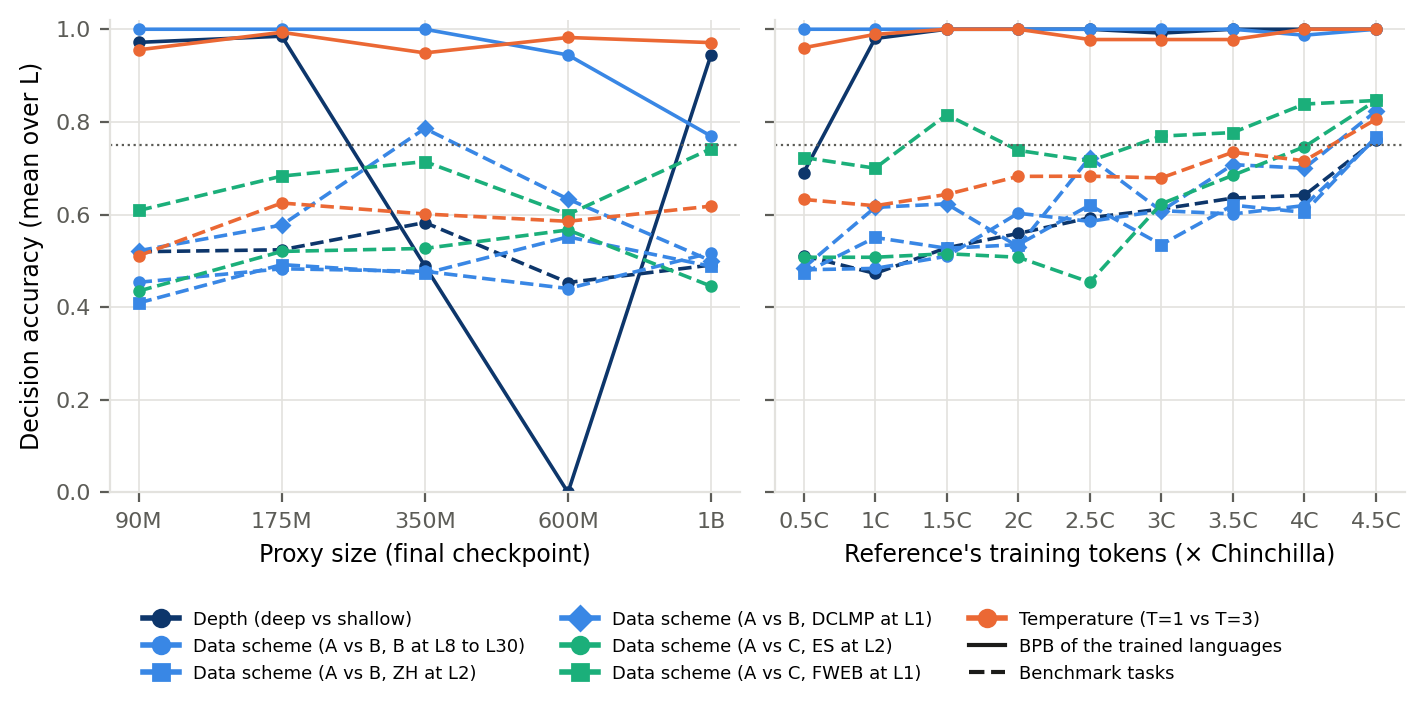
\includegraphics[width=\textwidth]{figures/app_design_decisions.png}
% source: src/signal-and-noise/analysis/rq05_design_decisions/pretraining/predictivity_seeds/da_all_lines_mono_axis_paper.png
\caption{Design decisions read by proxy size and by the reference's checkpoints.}
\label{fig:app_rq05_design_decisions}
\end{figure}
